\chapter{ĐẶT VẤN ĐỀ VÀ PHÂN TÍCH YÊU CẦU}

\section{Giới thiệu đề tài}
Trong bối cảnh nền kinh tế dịch vụ và du lịch phát triển mạnh mẽ trên phạm vi toàn cầu, ngành quản trị khách sạn và lưu trú đóng vai trò trụ cột. Đề tài 14: \textbf{``Dự đoán khách hàng hủy đặt phòng khách sạn (Hotel Booking Cancellation Prediction)''} được nghiên cứu nhằm áp dụng các kỹ thuật học máy có giám sát (Supervised Machine Learning) vào việc dự đoán khả năng khách hàng hủy phòng ngay từ thời điểm đặt phòng.

\section{Bối cảnh và ý nghĩa bài toán}
Phòng khách sạn là loại hàng hóa có hạn sử dụng ngắn hạn (Perishable Inventory) -- một đêm phòng nếu không được bán sẽ mất đi giá trị vĩnh viễn và không thể thu hồi. Khi khách hàng hủy đặt phòng đột ngột:
\begin{itemize}
    \item Doanh thu dự kiến bị sụt giảm nghiêm trọng.
    \item Khách sạn bị lãng phí nguồn lực chuẩn bị (nhân lực buồng phòng, thực phẩm).
    \item Nếu khách sạn áp dụng chiến lược đặt phòng vượt mức (Overbooking) quá cao mà không có mô hình định lượng, nguy cơ thiếu phòng sẽ gây ảnh hưởng tiêu cực đến uy tín thương hiệu.
\end{itemize}
Mô hình học máy dự báo sớm nguy cơ hủy giúp nhà quản trị tối ưu hóa kế hoạch kinh doanh và chính sách định giá động.

\section{Mục tiêu nghiên cứu}
\begin{enumerate}
    \item Khám phá và phân tích sâu các nhân tố ảnh hưởng đến quyết định hủy phòng từ dữ liệu thực tế.
    \item Thiết kế hai phương án tiền xử lý: Pipeline A (Cơ bản) và Pipeline B (Cải tiến với Kỹ thuật đặc trưng) đảm bảo tuyệt đối không xảy ra rò rỉ dữ liệu (No Data Leakage).
    \item Triển khai, tối ưu hóa và so sánh hiệu quả của các thuật toán: Baseline (DummyClassifier), K-Nearest Neighbors (KNN), Decision Tree (Cây quyết định).
    \item Đánh giá toàn diện mô hình trên tập kiểm thử độc lập thông qua nhiều chỉ số: Accuracy, Precision, Recall, F1-Score, ROC-AUC và phân tích ma trận nhầm lẫn.
    \item Thực hiện phân tích lỗi (False Positive và False Negative) nhằm đưa ra khuyến nghị thực tiễn cho nhà quản trị khách sạn.
\end{enumerate}

\section{Đối tượng nghiên cứu}
Đối tượng nghiên cứu là các giao dịch đặt phòng khách sạn được lưu vết trong hệ thống thông tin quản lý, bao gồm các thông tin về khách hàng, thời gian đặt trước, loại phòng, hình thức đặt cọc, số lượng khách và các yêu cầu đặc biệt.

\section{Phạm vi nghiên cứu}
Nghiên cứu tập trung vào bài toán Phân loại nhị phân (Binary Classification) với biến mục tiêu \texttt{is\_canceled} $\in \{0, 1\}$. Các dữ liệu trạng thái phát sinh sau khi đơn hàng kết thúc (như \texttt{reservation\_status}) bị loại trừ để bảo đảm tính thực tiễn khi ứng dụng mô hình tại thời điểm nhận đặt phòng.

\section{Giới thiệu bộ dữ liệu Hotel Booking Demand}
Nghiên cứu sử dụng bộ dữ liệu chuẩn mực \textbf{Hotel Booking Demand} của Jesse Mostipak \cite{mostipak2019kaggle}, bắt nguồn từ công trình nghiên cứu của Antonio, de Almeida và Nunes (2019) \cite{antonio2019hotel}.
\begin{itemize}
    \item \textbf{Quy mô:} 119,390 dòng quan sát và 32 thuộc tính.
    \item \textbf{Phạm vi khách sạn:} Gồm hai loại hình: Resort Hotel (H1, vùng Algarve) và City Hotel (H2, thành phố Lisbon, Bồ Đào Nha).
    \item \textbf{Khoảng thời gian:} Dữ liệu ghi nhận từ ngày 01/07/2015 đến ngày 31/08/2017.
\end{itemize}

\section{Mô tả các đặc trưng dữ liệu}
Bộ dữ liệu gồm 31 đặc trưng đầu vào và 1 biến mục tiêu:
\begin{itemize}
    \item \textbf{Đặc trưng thời gian:} \texttt{lead\_time}, \texttt{arrival\_date\_year}, \texttt{arrival\_date\_month}, \texttt{arrival\_date\_week\_number}, \texttt{arrival\_date\_day\_of\_month}, \texttt{stays\_in\_weekend\_nights}, \texttt{stays\_in\_week\_nights}.
    \item \textbf{Đặc trưng khách hàng:} \texttt{adults}, \texttt{children}, \texttt{babies}, \texttt{country}, \texttt{is\_repeated\_guest}, \texttt{customer\_type}.
    \item \textbf{Lịch sử đặt phòng:} \texttt{previous\_cancellations}, \texttt{previous\_bookings\_not\_canceled}, \texttt{booking\_changes}.
    \item \textbf{Đặc trưng thương mại:} \texttt{hotel}, \texttt{meal}, \texttt{market\_segment}, \texttt{distribution\_channel}, \texttt{reserved\_room\_type}, \texttt{assigned\_room\_type}, \texttt{deposit\_type}, \texttt{agent}, \texttt{company}, \texttt{days\_in\_waiting\_list}, \texttt{adr}, \texttt{required\_car\_parking\_spaces}, \texttt{total\_of\_special\_requests}.
\end{itemize}

\section{Phân tích khám phá dữ liệu (EDA)}
Quá trình phân tích khám phá dữ liệu trên toàn bộ 119,390 dòng quan sát đã xác định các đặc điểm phân phối quan trọng:
\begin{itemize}
    \item \textbf{Tỷ lệ hủy phòng theo khách sạn:} City Hotel có tỷ lệ hủy lên đến $41.73\%$ (33,102 đơn hủy trên 79,330 đơn), trong khi Resort Hotel có tỷ lệ hủy là $27.76\%$ (11,122 đơn hủy trên 40,060 đơn).
    \item \textbf{Tác động của hình thức đặt cọc (\texttt{deposit\_type}):} Đáng lưu ý, nhóm đặt cọc không hoàn lại (\texttt{Non Refund}) có tỷ lệ hủy lên tới $99.36\%$ (14,494 đơn hủy trên 14,587 đơn). Đây là các hợp đồng đặt theo đoàn hoặc đại lý mà chính sách buộc ghi nhận trạng thái hủy khi đoàn không đến.
    \item \textbf{Thời gian đặt trước (\texttt{lead\_time}):} Khách đặt trước càng sớm thì tỷ lệ hủy càng cao (đơn đặt trên 1 năm có tỷ lệ hủy trên $70\%$, trong khi đơn đặt trong vòng 1 tuần chỉ có tỷ lệ hủy dưới $15\%$).
    \item \textbf{Yêu cầu đặc biệt (\texttt{total\_of\_special\_requests}):} Khách hàng có từ 2 yêu cầu đặc biệt trở lên có tỷ lệ hủy dưới $22\%$, thấp hơn nhiều so với khách không có yêu cầu nào ($47.7\%$).
\end{itemize}

\begin{figure}[H]
    \centering
    \begin{subfigure}{0.48\textwidth}
        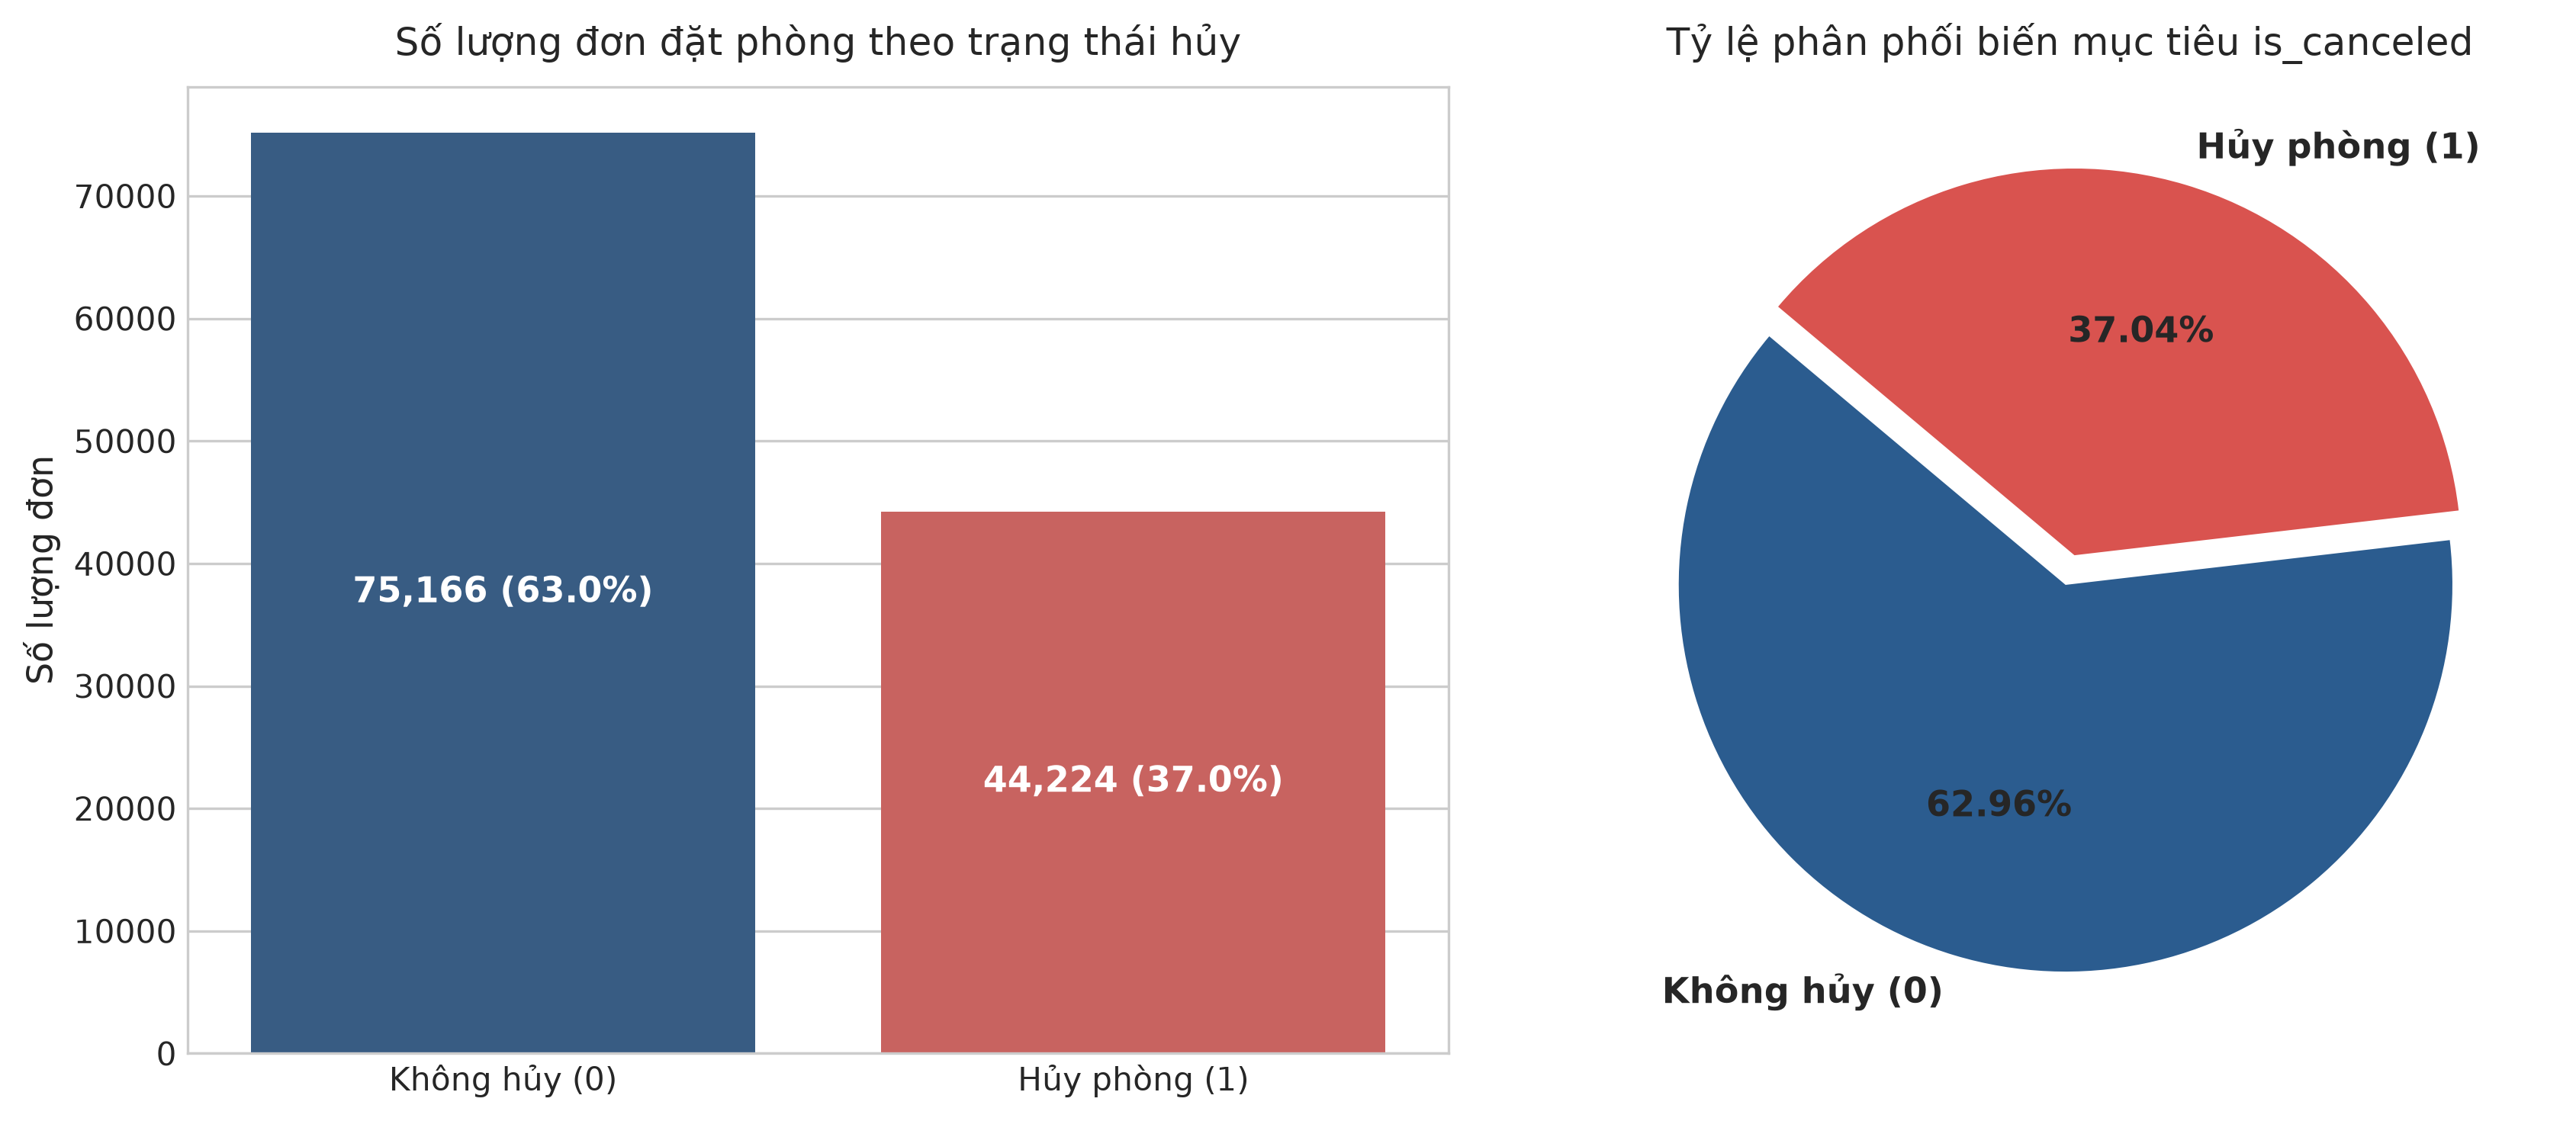
\includegraphics[width=\linewidth]{01_target_distribution.png}
        \caption{Phân phối biến mục tiêu \texttt{is\_canceled}}
    \end{subfigure}
    \begin{subfigure}{0.48\textwidth}
        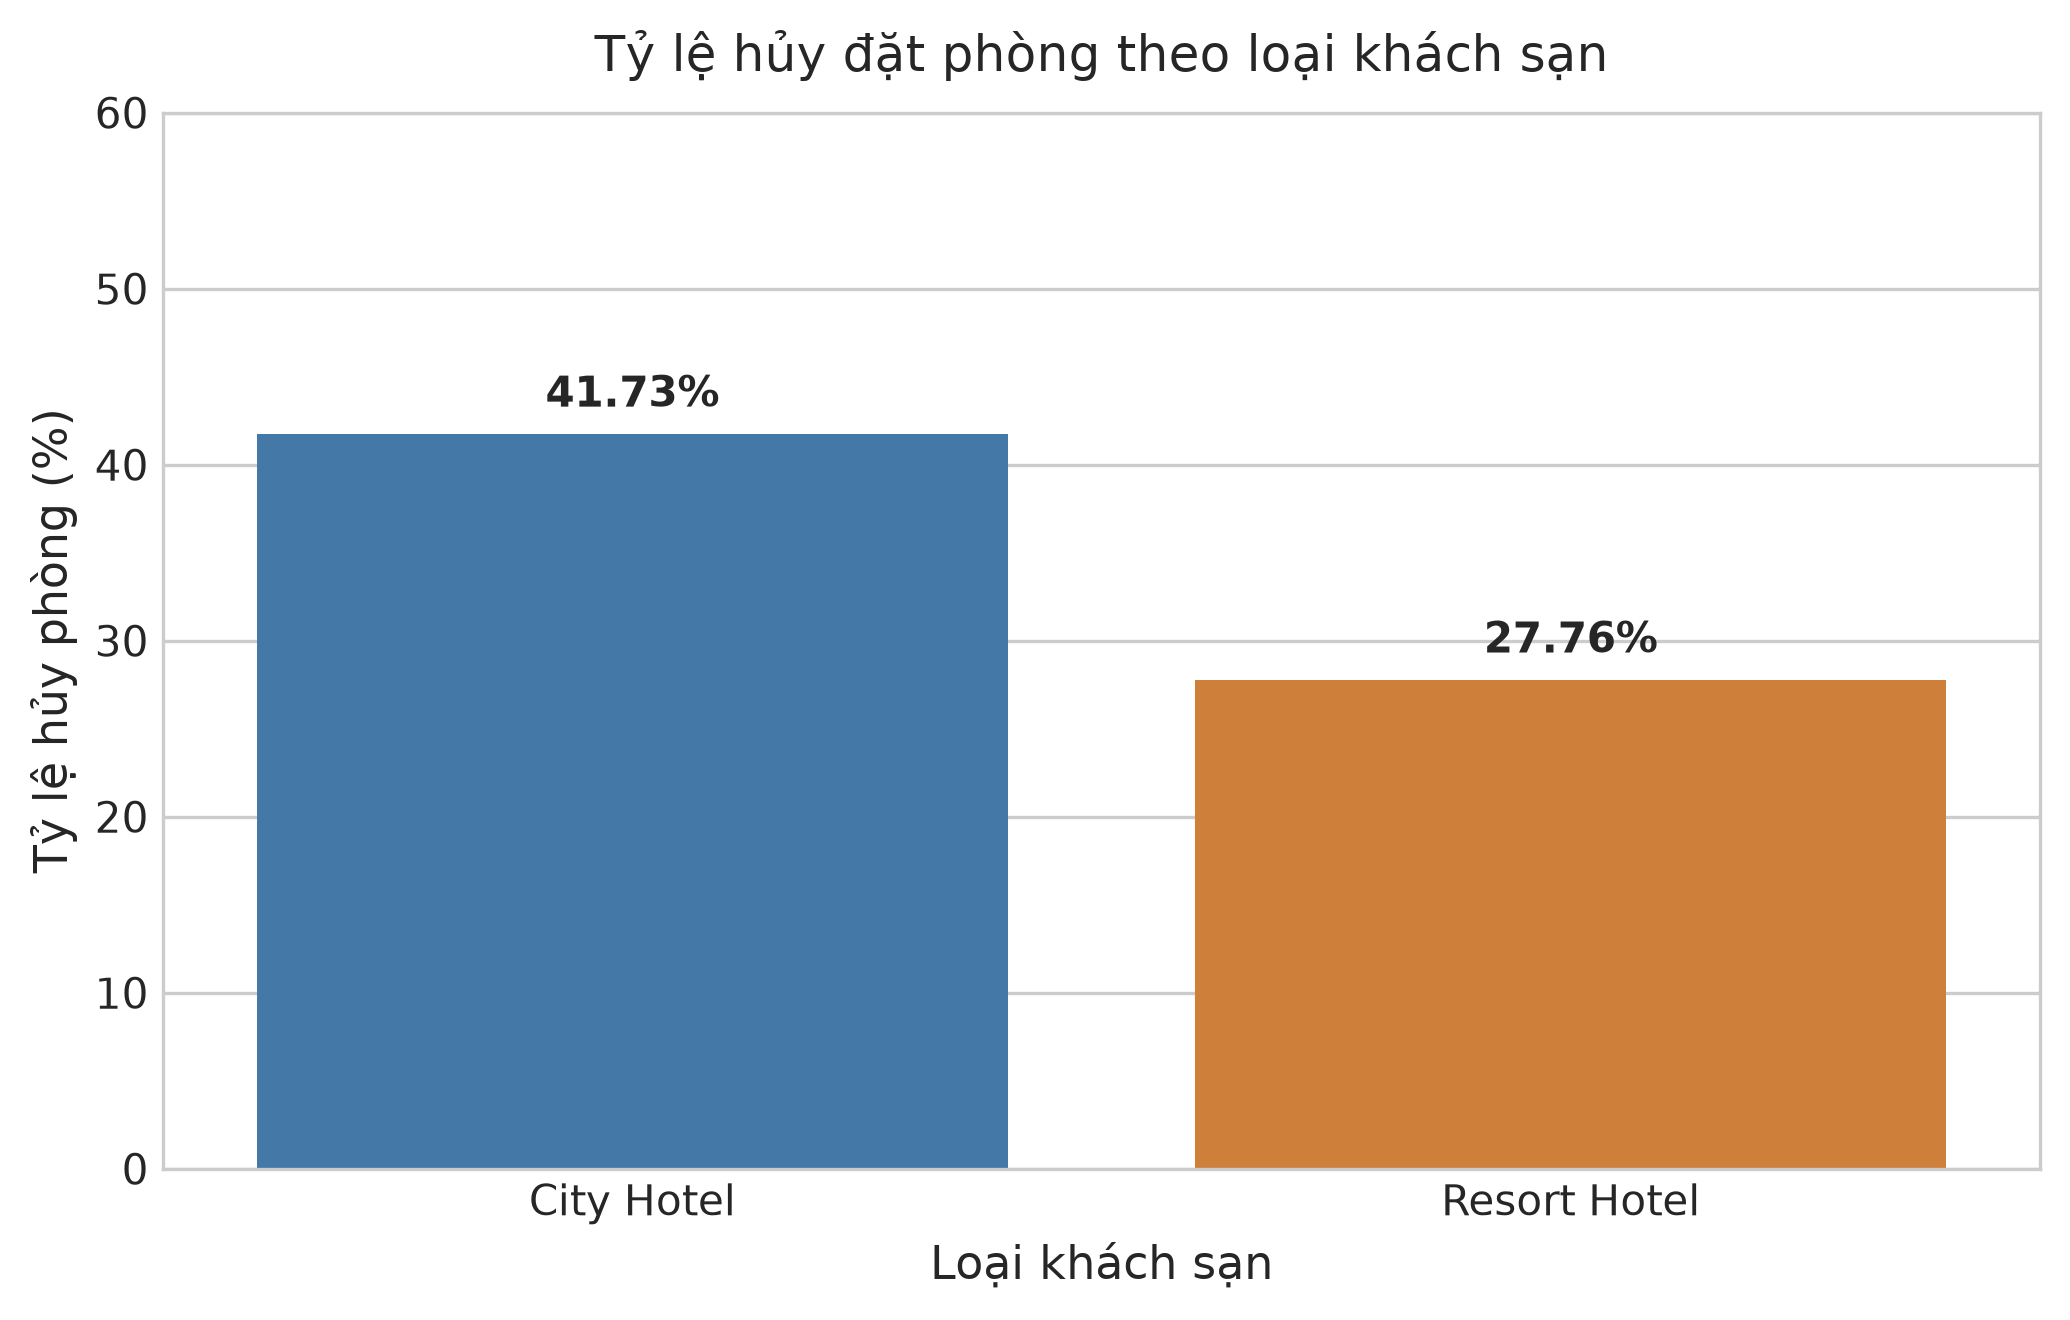
\includegraphics[width=\linewidth]{03_cancellation_by_hotel.png}
        \caption{Tỷ lệ hủy theo loại khách sạn}
    \end{subfigure}
    \caption{Phân tích phân phối mục tiêu và loại hình khách sạn}
    \label{fig:eda_overview}
\end{figure}

\begin{figure}[H]
    \centering
    \begin{subfigure}{0.48\textwidth}
        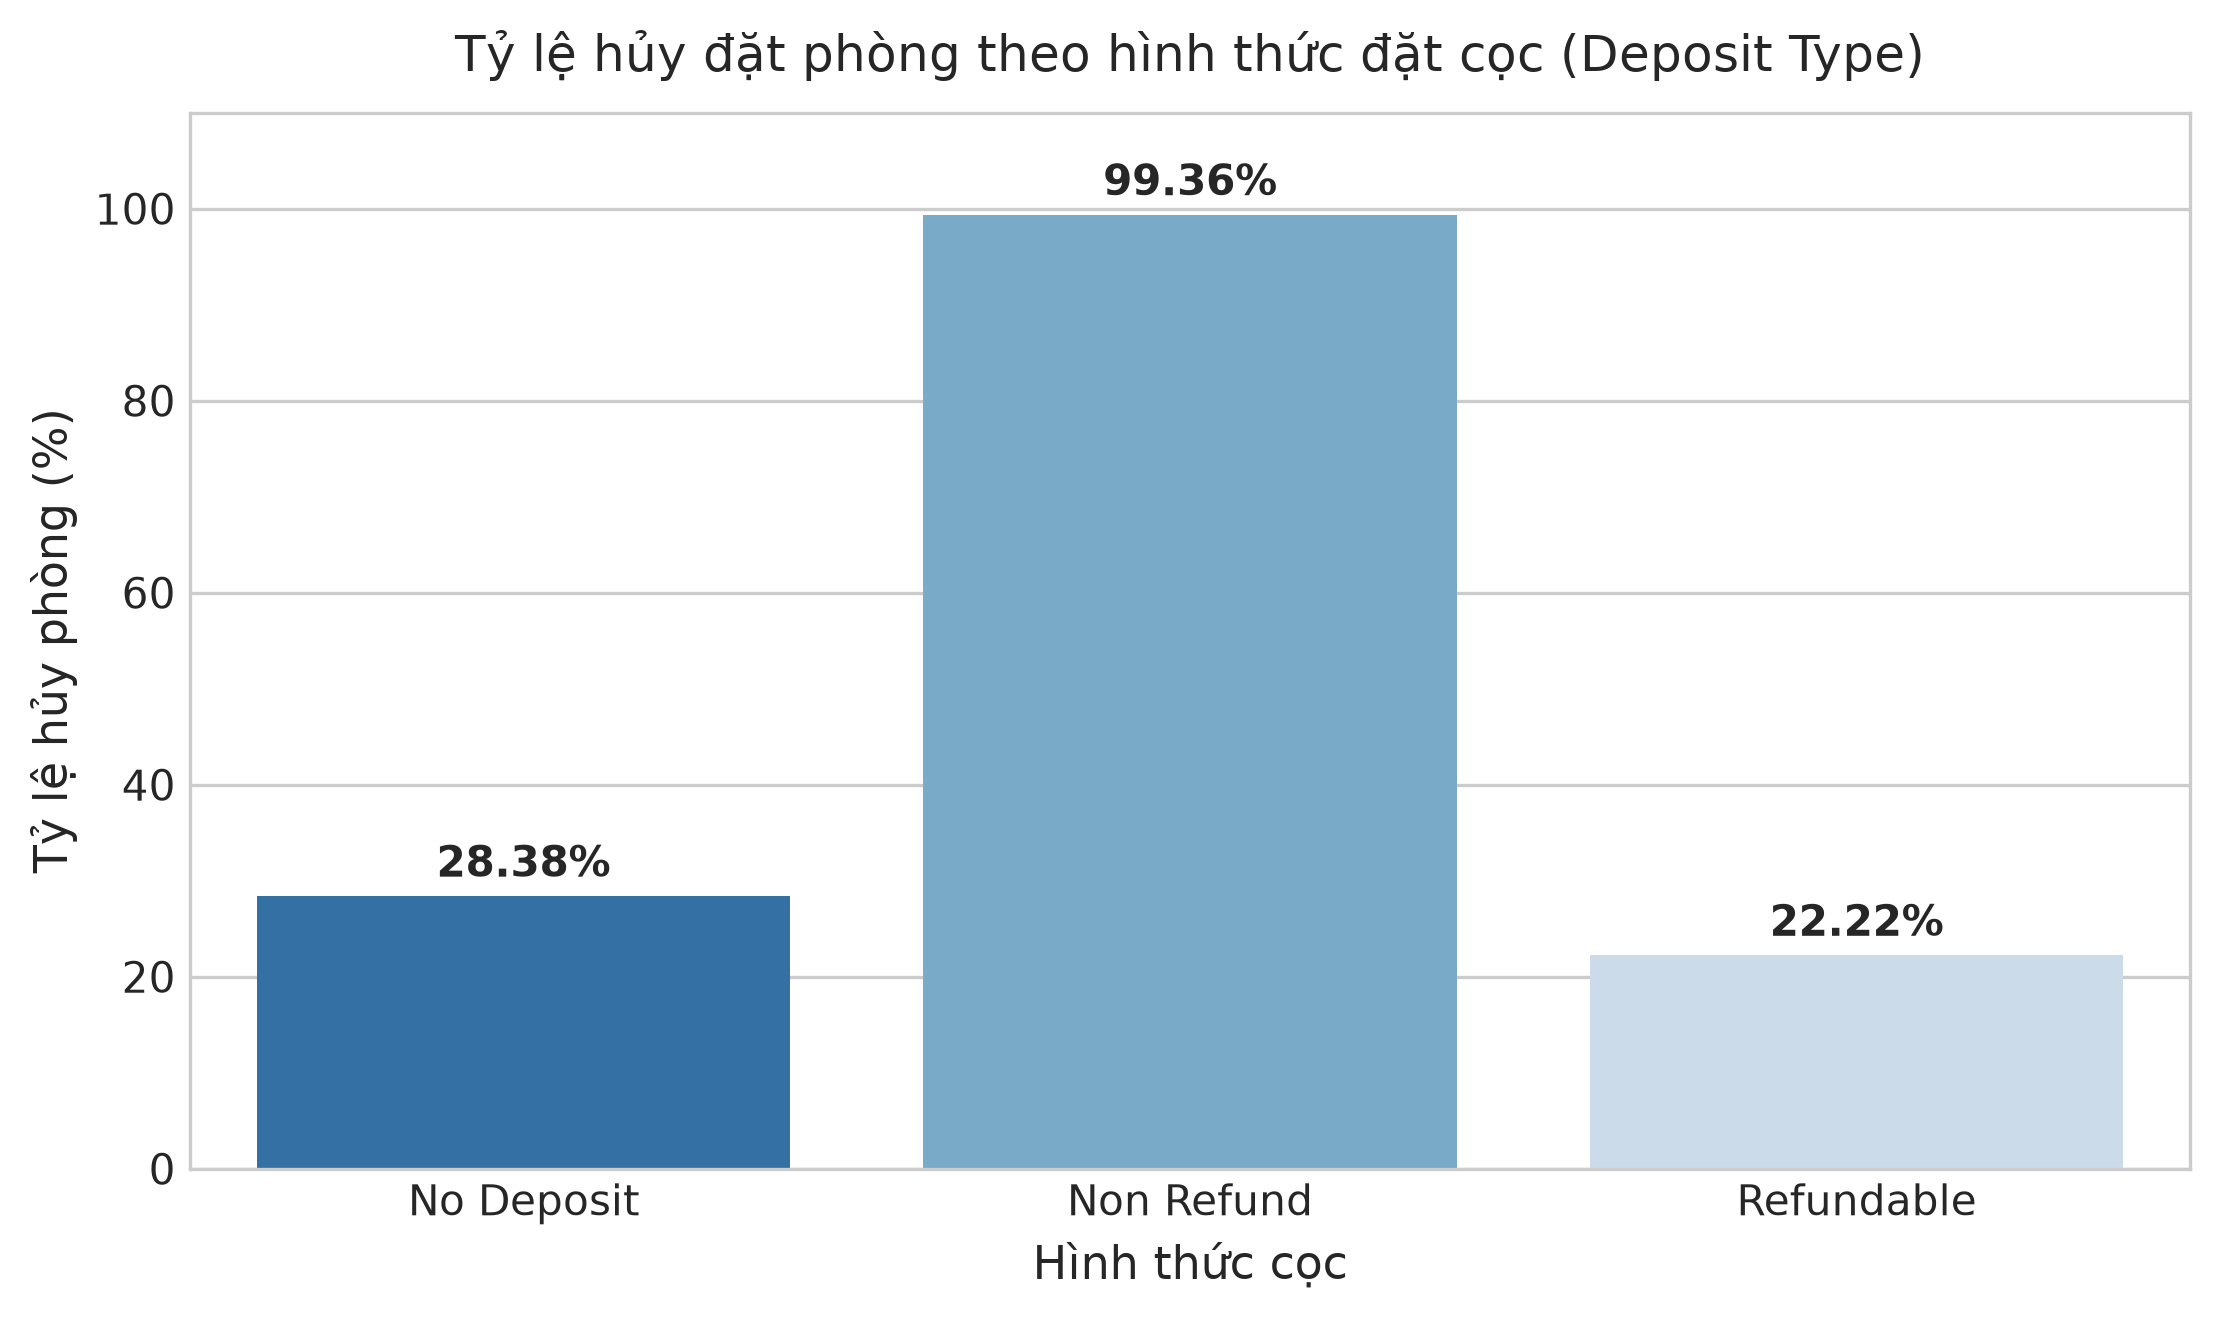
\includegraphics[width=\linewidth]{04_cancellation_by_deposit_type.png}
        \caption{Tỷ lệ hủy theo hình thức đặt cọc}
    \end{subfigure}
    \begin{subfigure}{0.48\textwidth}
        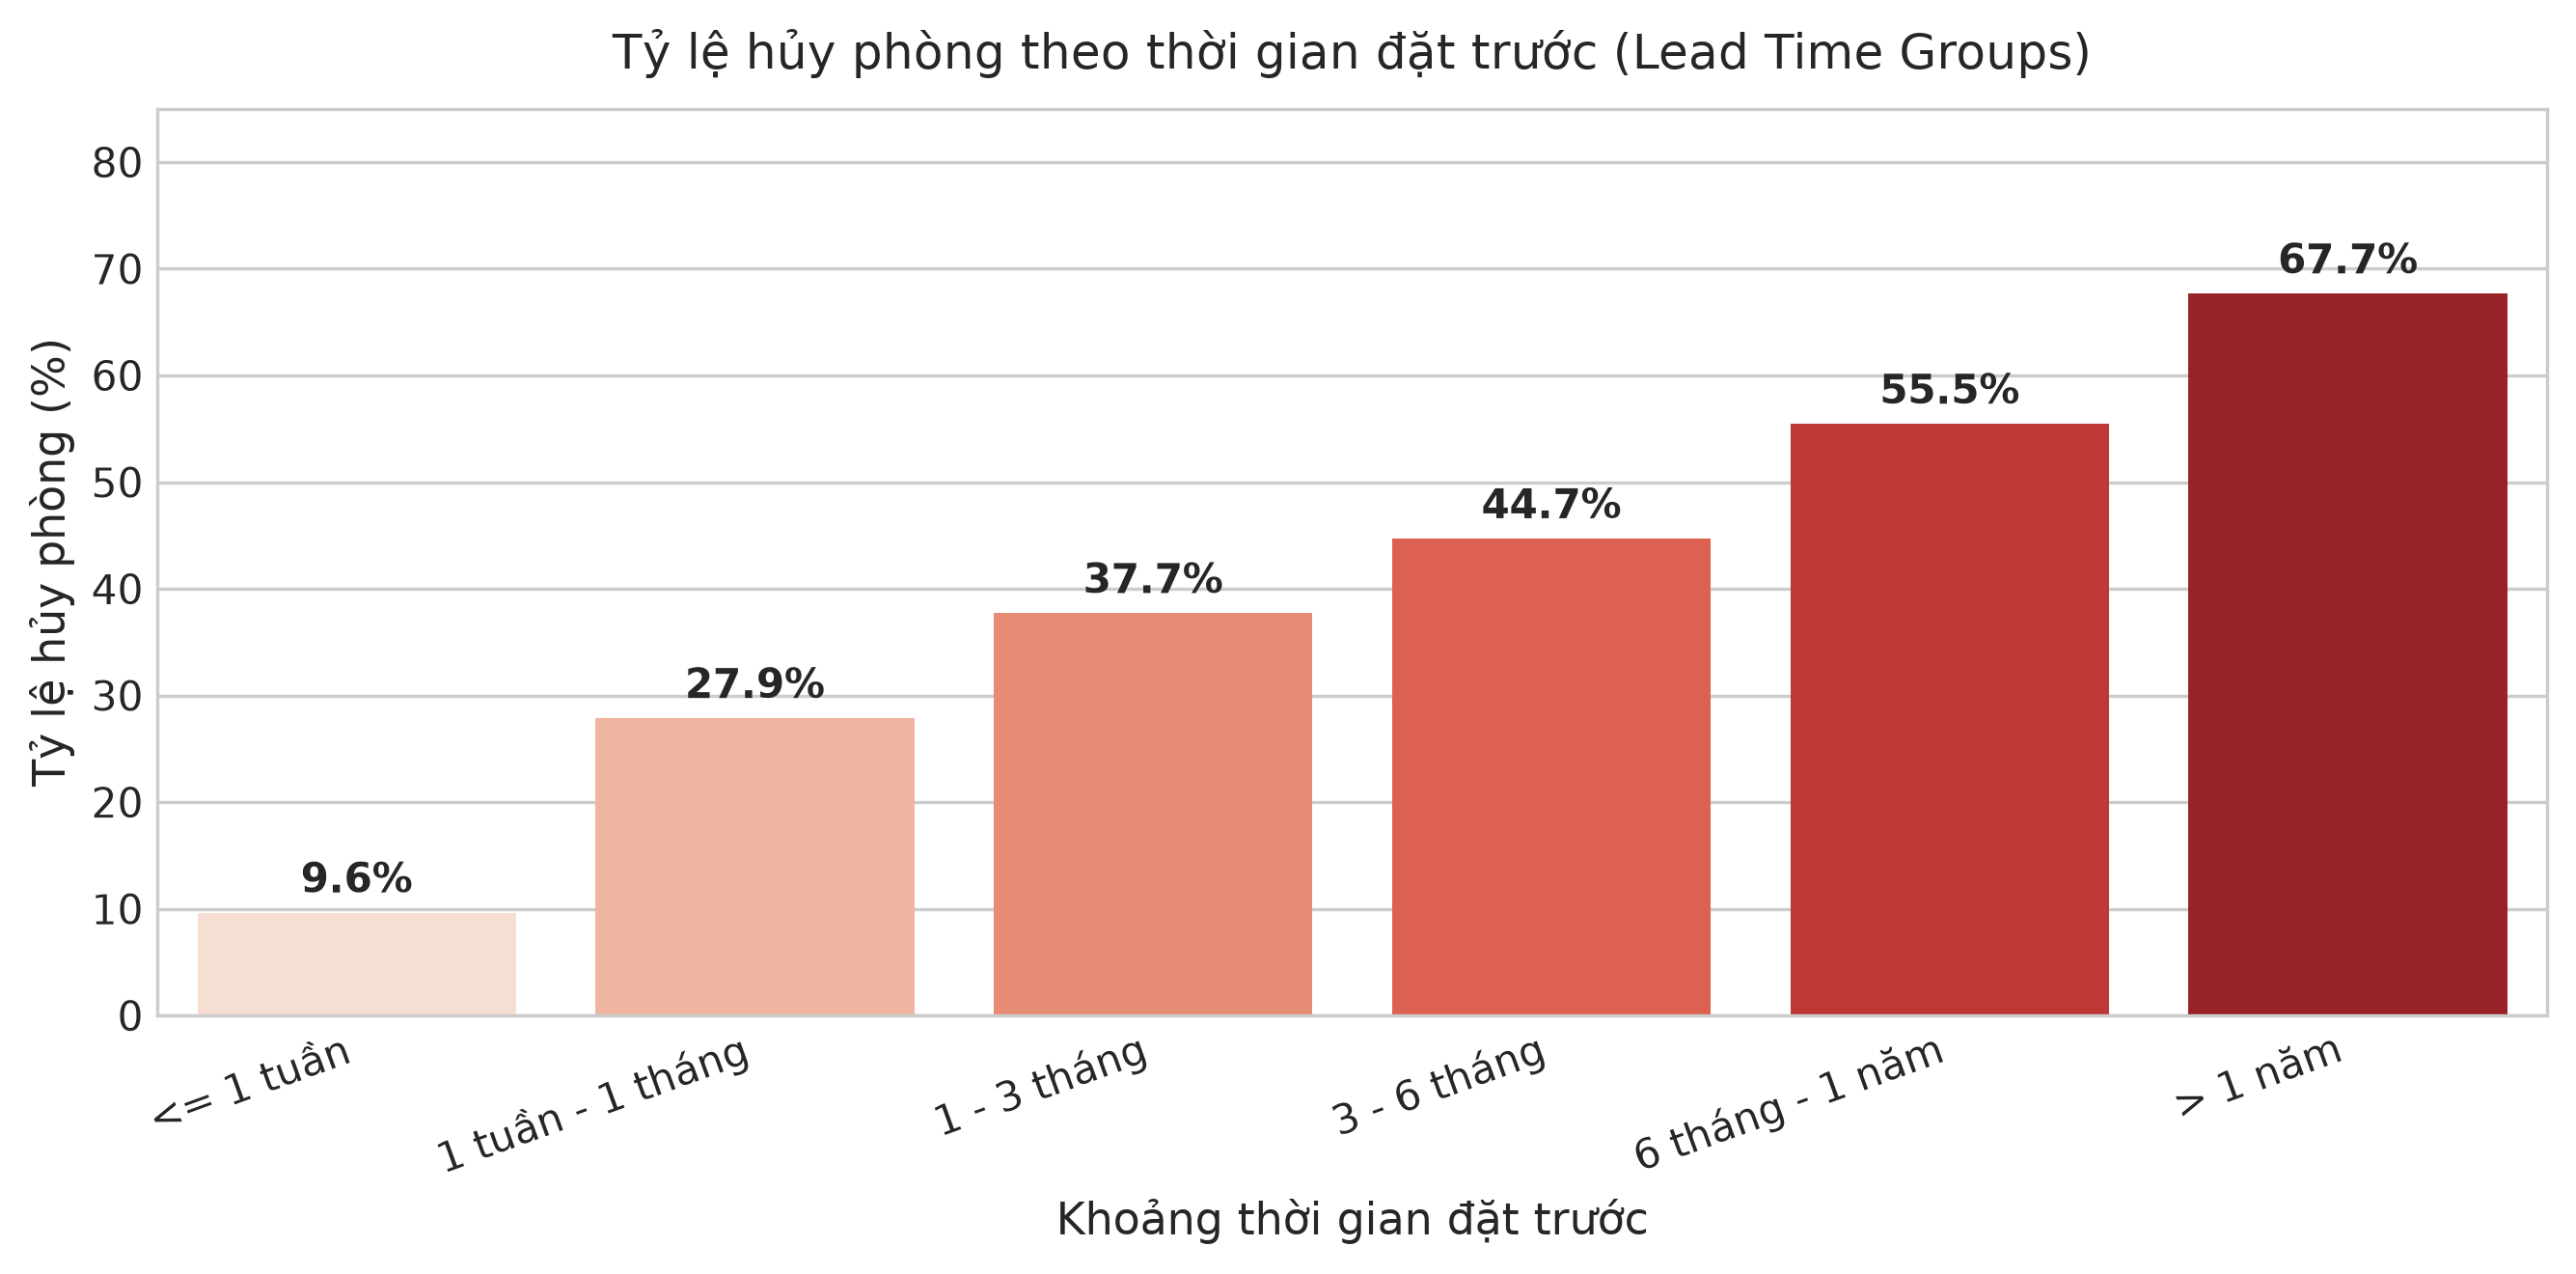
\includegraphics[width=\linewidth]{07_cancellation_by_lead_time_group.png}
        \caption{Tỷ lệ hủy theo khoảng thời gian đặt trước}
    \end{subfigure}
    \caption{Mối quan hệ giữa đặt cọc, thời gian đặt trước và nguy cơ hủy phòng}
    \label{fig:eda_relationships}
\end{figure}

\section{Phân tích biến mục tiêu}
Biến mục tiêu \texttt{is\_canceled} có phân phối thực tế như sau:
\begin{itemize}
    \item Lớp 0 (Khách nhận phòng, không hủy): 75,166 mẫu, chiếm $62.96\%$.
    \item Lớp 1 (Khách hủy phòng hoặc No-Show): 44,224 mẫu, chiếm $37.04\%$.
\end{itemize}
Bộ dữ liệu có độ mất cân bằng nhẹ (tỷ lệ xấp xỉ $1.7 : 1$). Do đó, việc chia dữ liệu cần sử dụng kỹ thuật Stratified Split, và việc đánh giá mô hình không thể chỉ dựa vào Accuracy mà bắt buộc phải sử dụng Precision, Recall và F1-Score.

\section{Các vấn đề phát hiện từ dữ liệu}
\begin{enumerate}
    \item \textbf{Dữ liệu thiếu (Missing Data):}
    \begin{itemize}
        \item \texttt{company}: Thiếu 112,593 giá trị ($94.31\%$).
        \item \texttt{agent}: Thiếu 16,340 giá trị ($13.69\%$).
        \item \texttt{country}: Thiếu 488 giá trị ($0.41\%$).
        \item \texttt{children}: Thiếu 4 giá trị ($0.003\%$).
    \end{itemize}
    \item \textbf{Dữ liệu trùng lặp:} 31,994 dòng ($26.8\%$) có giá trị các thuộc tính trùng nhau hoàn toàn do không có trường định danh cá nhân (ID). Nhóm giữ nguyên tập dữ liệu này để phản ánh đúng phân phối tần suất đặt phòng ngoài thực tế.
    \item \textbf{Giá trị ngoại lệ và dị thường:} Phát hiện 1 dòng có giá phòng trung bình $\text{ADR} = -5.4$ và 180 dòng có tổng số khách bằng 0 (\texttt{adults} + \texttt{children} + \texttt{babies} = 0).
    \item \textbf{Nguy cơ rò rỉ dữ liệu (Data Leakage):} Hai cột \texttt{reservation\_status} và \texttt{reservation\_status\_date} chứa thông tin sau khi giao dịch kết thúc, bắt buộc phải loại bỏ trước khi xây dựng mô hình.
\end{enumerate}
